	\pagecolor{goban}
\thispagestyle{empty}
\begin{center}
	\vspace*{1cm} 
	\begin{tikzpicture}
		\node[font=\fontsize{180}{156}\bfseries\selectfont, text=black] at (0,0) {圍道};
		
	\end{tikzpicture}
	%		\begin{tikzpicture}
		%			\node[font=\fontsize{196}{156}\bfseries\selectfont, text=black] at (0,0) {圍};
		%			\node[font=\fontsize{196}{156}\bfseries\selectfont, text=black] at (0,-8) {道};
		%		\end{tikzpicture}
	\vspace{1.5cm}
	
	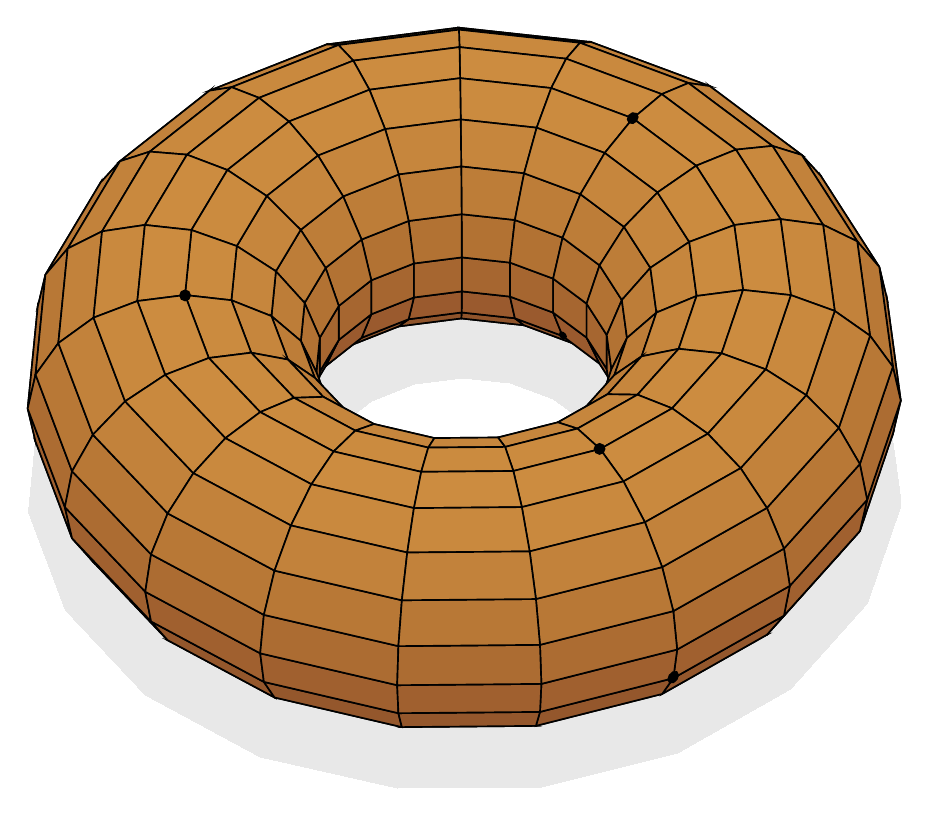
\begin{tikzpicture}[scale=3]
		\pgfplotsset{
			colormap={teak}{
				rgb=(0.5,0.3,0.15)
				rgb=(0.6,0.35,0.18)
				rgb=(0.7,0.45,0.2)
				rgb=(0.8,0.55,0.25)
			},
			% New colormap specifically for the shadow
			colormap={shadow}{
				gray=(0.1)
				gray=(0.1)
			}
		}
		\begin{axis}[
			hide axis,
			view={4}{45},
			axis equal image,
			samples=20,
			domain=0:360,
			y domain=0:360,
			z buffer=sort,
			]
			
			% 1. Sombra
			\addplot3[
			surf,
			shader=interp,
			draw=none,     
			colormap name=shadow,
			opacity=0.1
			]
			(
			{(2 + cos(y)) * cos(x)},
			{(2 + cos(y)) * sin(x)},
			{-1} 
			);
			
			% 2. toro
			\addplot3[
			surf,
			shader=flat,
			draw=black,
			colormap name=teak,
			line width=0.2pt,
			opacity=1
			]
			(
			{(2 + cos(y)) * cos(x)},
			{(2 + cos(y)) * sin(x)},
			{sin(y)}
			);
			
			%%%%%%%%%%%%%%%%%%%%  puntos negros
			\addplot3[
			only marks,
			xslant=-0.15,
			yslant=-0.5,
			mark options={shading=ball, ball color=white},
			mark size=0.25pt,
			shading=ball,
			color=black
			] coordinates {(1.190, 3.94, 0)};
			
			\addplot3[
			only marks,
			mark options={shading=ball, ball color=white},
			mark size=0.5pt,
			shading=ball,
			color=black
			] coordinates {(-1.96, 0.675, 0)};
			
			\addplot3[ %centro
			only marks,
			mark options={shading=ball, ball color=white},
			mark size=0.5pt,
			shading=ball,
			color=black
			] coordinates {(0.975, -0.61, 0)};
			
			\addplot3[ %arriba derecha
			only marks,
			yslant=0.25,
			mark options={shading=ball, ball color=white},
			mark size=0.5pt,
			shading=ball,
			color=black
			] coordinates {(1.09, 1, 0)};
			
			\addplot3[ %abajo derecha
			only marks,
			yslant=0.5,
			mark options={shading=ball, ball color=black},
			mark size=0.5pt,
			shading=ball,
			color=black
			] coordinates {(1.870,-6.179, 0)};
		\end{axis}
	\end{tikzpicture}
	\vspace{1cm}
	
	% 2. Aplicación de la fuente al título
	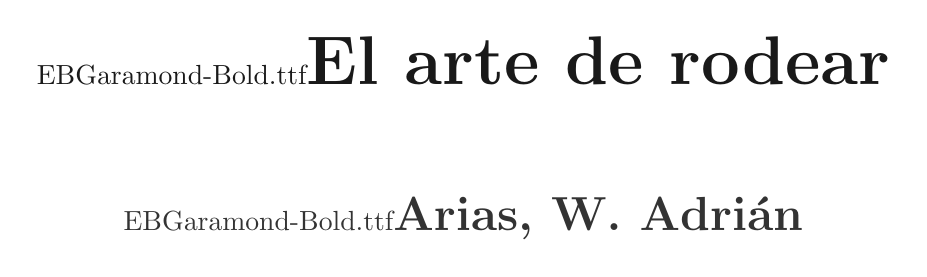
\begin{tikzpicture}
		% Changes the node to Helvetica
		\node[font=\fontspec{EBGaramond-Bold.ttf}\fontsize{24}{156}\bfseries\selectfont, text=black!90] at (0,0) {El arte de rodear};
		\node[font=\fontspec{EBGaramond-Bold.ttf}\fontsize{16}{156}\bfseries\selectfont, text=black!80] at (0,-2) {Arias, W. Adrián};
	\end{tikzpicture}
	
	
\end{center}
\newpage
%%%%%%%%% PORTADA

\pagecolor{white}
\thispagestyle{empty}
\clearpage

\thispagestyle{empty}
\maketitle
% --- FORZAR ESTILO EN PÁGINAS DE CAPÍTULO ---
% Redefinimos el estilo 'plain' que LaTeX usa automáticamente al iniciar capítulos
\clearpage
\thispagestyle{empty}

\vspace*{0.2925\textheight} % Ajuste para el »Centro Óptico» (más arriba que el centro)

\begin{center}
	% Usamos un ancho similar al del bloque del poema (ej. 7.5cm o 8cm)
	% para que el »peso» visual del cuadrado de la foto sea igual al del texto.
	%		
\includegraphics[width=7.5cm]{ipe_mitad.jpg}
	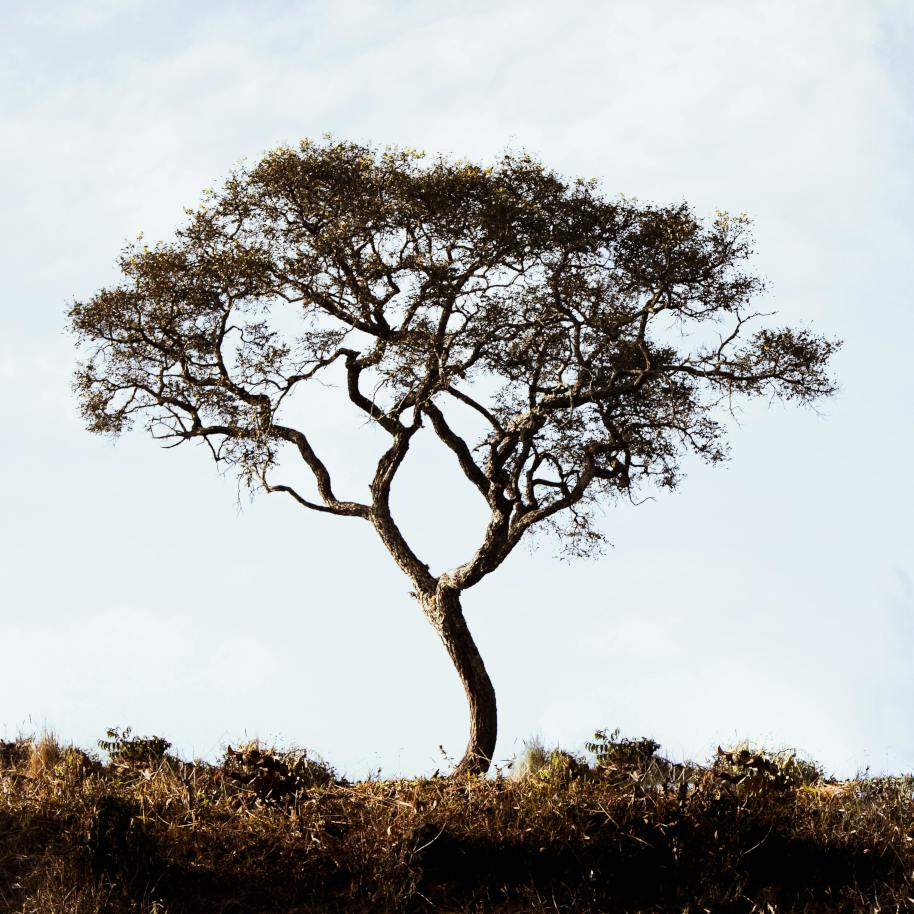
\includegraphics[width=7.5cm]{figures/ipe_cuarto.jpg}
\end{center}

\vspace*{\fill} % Empuja desde abajo
\clearpage
\thispagestyle{empty} % Esto quita encabezados, pies y números de esta página
\vspace*{0.3\textheight} % Ajuste para el »Centro Óptico» (más arriba que el centro)

\begin{center}
	\begin{minipage}{6.375cm}
		\linespread{1.3}\selectfont
		\itshape
		Contemplo o rio que corre parado \\
		E a dançarina de pedra que evolui \\
		Completamente, sem metas, sentado \\
		Não tenho sido, não sou, não serei, nem fui \\
		A mente quer ser, mas querendo erra \\
		Pois só sem desejos é que se vive o agora\\
		Vêde o pé do ypê, apenasmente flora\\
		Revolucionariamente\\
		Apenso ao pé da serra
		
		\vspace{1.5em}
		\hfill \upshape  --- \textbf{Belchior} «Ypê»
	\end{minipage}
\end{center}
\vfill % Empuja todo hacia arriba
\clearpage
\thispagestyle{empty}
\section*{Prefacio}
\thispagestyle{empty}
What's Go? A game, of course. But one might ask: How is it done precisely?, What can be done and what not? Is it possible to extend it's concepts to other games?


\textit{圍道 — Wéi Dào — El arte de rodear} (The art of sorrounding but we choose The art of Go as the english title) Tries to answer such questions by constructing a rigurous theory of the game of Go, follow by it's generalization in and out of the table.

This work it's separated in three parts as follows:

\textbf{Parte I: Foundation.} We beging the study of the game by it's history, starting in ancient China to it's origin into Argentina. We finish this part with the rules of the game and setting the construction motivation.


\textbf{Parte II: Construction.} Now that we know the game we are ready to build it formally. The two dimensional version of the game it's constructed. It's defined the board, the pieces, the colors, the relations between them. The concept of group, captures, SuperKo are defined. The legallity of a play it's formalized via a theorem of when a play it's legal. The SuperKo detection it's handled by Zobrist Hashing. The whole srtuctured it's name a Go and we begin to generalized it. Finally we discuss the \textit{life in the game of go} by 

Una vez comprendido el juego, se construye formalmente un modelo en dos dimensiones y dos jugadores. Se definen con precisión las nociones de jugada legal, captura y SuperKo (resuelto mediante hashing de Zobrist), y posteriormente se generaliza el marco a $n$ dimensiones y $m$ jugadores. Finalmente, se estudia la noción de \textit{vida} dentro del juego, partiendo del trabajo de Benson, incorporando la vida condicional y presentando una observación a un teorema de Bai.

\textbf{Parte III: Abstracciones.} Establecidas las bases, el estudio se vuelca hacia afuera. Se analiza el comportamiento de las adyacencias en dimensiones superiores, donde se evidencia que el Go tridimensional pierde el equilibrio y traiciona la esencia del juego original. También se estudia el caso unidimensional y, finalmente, se busca un origen común para estos juegos y otros aparentemente distintos.

\vfill

Quisiera agradecer a Gusti Cabaña por ser mi primer lector y darme una dirección cuando menos la tenía. También a Diego Barrios y Eros Girardi, por leer el trabajo y darme muy útiles comentarios. Finalmente a Naza, por aguantarme todo estos años.
\clearpage

\tableofcontents
\thispagestyle{empty}
\clearpage